%\documentclass[12pt, hyperref={pdfpagemode=FullScreen} ]{beamer}
\documentclass[12pt]{beamer}

\usepackage{array}
\usepackage{color}
\usepackage{listings}
\usepackage{minted}
\usemintedstyle{autumn}


\renewcommand{\theFancyVerbLine}{\sffamily
\textcolor[rgb]{0.5,0.5,1.0}{\scriptsize
\oldstylenums{\arabic{FancyVerbLine}}}}


\mode<presentation>
{
	%\usetheme{Warsaw}
	%\usetheme{Darmstadt}
	\usetheme{Boadilla}
	%\usetheme{CambridgeUS}
	%\usetheme{Madrid}
}

\makeatletter
\setbeamertemplate{footline}
{
  \leavevmode%
  \hbox{%
  \begin{beamercolorbox}[wd=.333333\paperwidth,ht=2.25ex,dp=1ex,center]{author in head/foot}%
    \usebeamerfont{author in head/foot}\insertshortauthor%~~\beamer@ifempty{\insertshortinstitute}{}{(\insertshortinstitute)}
  \end{beamercolorbox}%
  \begin{beamercolorbox}[wd=.333333\paperwidth,ht=2.25ex,dp=1ex,center]{title in head/foot}%
    \usebeamerfont{title in head/foot}\insertshorttitle
  \end{beamercolorbox}%
  \begin{beamercolorbox}[wd=.333333\paperwidth,ht=2.25ex,dp=1ex,right]{date in head/foot}%
    \usebeamerfont{date in head/foot}\insertshortdate{}\hspace*{2em}
    \insertframenumber{} / \inserttotalframenumber\hspace*{2ex} 
  \end{beamercolorbox}}%
  \vskip0pt%
}
\makeatother



\def\newblock{\hskip .11em plus.33em minus.07em} %to solve a beamer problem with bib files

\usepackage{times}
\usepackage{tikz}
\usepackage{verbatim}
\usetikzlibrary{arrows,shapes}
\usepackage{natbib} 


\setbeamertemplate{navigation symbols}{
   %\insertslidenavigationsymbol
   %\insertframenavigationsymbol
   %\insertsubsectionnavigationsymbol
   %\insertsectionnavigationsymbol
   %\insertdocnavigationsymbol
   %\insertbackfindforwardnavigationsymbol
}
\title[Ruby on Rails]{Introduction to Ruby on Rails as an ORM}
\date{}
\institute{}
\author{Pierre-Yves Dupont}
\begin{document}


\newcommand{\mynewsection}[1]{
\section{#1}
\subsection*{}
\begin{frame}
	\begin{block}{}
		\center{#1}
	\end{block}
\end{frame}
}

\begin{frame}
	\titlepage
\end{frame}

\mynewsection{Simple example}

\begin{frame}
\vspace{-1.2cm}
	\begin{figure}	
		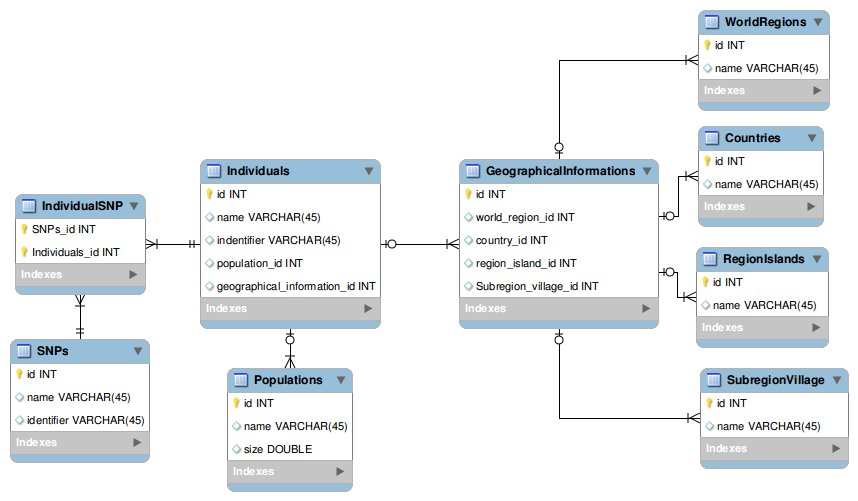
\includegraphics[scale=0.30]{dbscheme.png}
	\end{figure}
	\begin{block}{}
		\only<1>{
			\emph{Individuals} is a \textbf{Table}, having many \textbf{attributes} like \emph{name}
		}
		\only<2>{
			Individuals \textbf{belongs to} a Population\\
			
		}
		\only<3>{
			Population \textbf{has many} Individuals\\ 
		}
		\only<4>{
			Individuals \textbf{has many} SNPs \\
			SNPs \textbf{has many} Individuals
		}
		\only<5>{
			Individuals \textbf{has and belongs to many} SNPs\\
			nn relation
		}
	\end{block}
\end{frame}

\mynewsection{Design Pattern MVC}

\begin{frame}
	\begin{figure}{MVC: Model View Controller}
		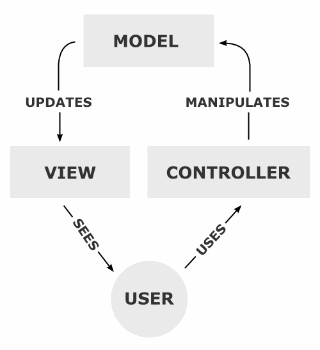
\includegraphics[scale=0.50]{MVC-Process.png}
	\end{figure}
\end{frame}

\begin{frame}[fragile]
	\begin{figure}{MVC: in RoR}
		\centering{
		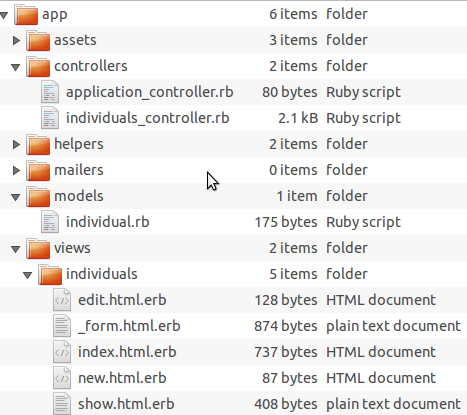
\includegraphics[scale=0.50]{TreeRails.png}
		}
	\end{figure}
\end{frame}

\mynewsection{Ruby on Rails ORM}

\begin{frame}[fragile]
  \begin{block}{ActiveRecod Models}
	\begin{minted}[fontsize=\scriptsize, linenos=true, numbersep=5pt]{ruby}
#In app/models/individual.rb file
class Individual < ActiveRecord::Base
  attr_accessible :identifier, :name
  belongs_to :population
  belongs_to :geographical_information
  has_and_belongs_to_many :snps
end

#In app/models/population.rb file
class Population < ActiveRecord::Base
  attr_accessible :name, :size
  has_many :individuals
end
	\end{minted}
  \end{block} 
\end{frame}

\begin{frame}[fragile]
  \begin{block}{Database link}
  	Convention over configuration (software design paradigm)
	\begin{minted}[fontsize=\scriptsize, linenos=true, numbersep=5pt]{ruby}
#In app/models/individual.rb file
#Model Individual -> table individuals
class Individual < ActiveRecord::Base
  #Attributes -> fields in the table
  attr_accessible :identifier, :name
  #population_id field in individuals table
  belongs_to :population 
  belongs_to :geographical_information
  #join table individuals_populations
  has_and_belongs_to_many :snps
end
	\end{minted}
  \end{block} 
\end{frame}

\begin{frame}[fragile]
  \begin{block}{Database link}
  	Some necessary configuration \ldots
	\begin{minted}[fontsize=\scriptsize, linenos=true, numbersep=5pt]{yaml}
#In config/database.yml
development:
  adapter: mysql2
  encoding: utf8
  reconnect: false
  database: tutorails_development
  pool: 5
  username: root
  password: atadxam
  socket: /var/run/mysqld/mysqld.sock
	\end{minted}
  \end{block} 
\end{frame}

\begin{frame}[fragile]
  \begin{block}{Python ORM (SQLAlchemy)}
	\begin{minted}[fontsize=\scriptsize, linenos=true, numbersep=5pt]{python}
class Individuals(Base):
    __tablename__ = 'individuals'
 
    id = Column(Integer, primary_key=True)
    name = Column(String(255), nullable=False)
    identifier = Column(Integer,nullable=False)
    population_id = Column(Integer,ForeignKey('population.id'))
    population = relation("Population", backref='individuals')
 
    def __init__(self, title=None, year=None):
        self.title = title
        self.year = year
	\end{minted}
  \end{block} 
\end{frame}

\mynewsection{Querying the database}

\begin{frame}[fragile]
  \begin{block}{Simple queries}
	\begin{minted}[fontsize=\scriptsize, linenos=true, numbersep=5pt]{ruby}
Population.all

Population.first

Population.last

Population.order("size desc").limit(10)

Population.where("size <= ?", 1000).includes(:individuals)

Population.order("size").last

Population.first.name

Population.first.individuals
	\end{minted}
  \end{block}  
\end{frame}

\begin{frame}[fragile]
  \begin{block}{Defining a scope (subset)}
	\begin{minted}[fontsize=\scriptsize, linenos=true, numbersep=5pt]{ruby}
class Population < ActiveRecord::Base
  attr_accessible :name, :size
  has_many :individuals
  
  #static method Population.smaller_than(1)
  def self.smaller_than(x)
    where("populations.size < ?", x)
  end

  #definition of the scope small
  scope :small, smaller_than(1000)
  #definitions of individuals belonging to ``Foo'' population
  scope :foos, joins(:population).\
  	where('populations.name LIKE "Foo"')
end
	\end{minted}
  \end{block}
  \begin{block}{}
	\begin{minted}[fontsize=\scriptsize]{bash}
%> Population.small
	\end{minted}
  \end{block}
  \begin{block}{}
	\begin{minted}[fontsize=\scriptsize]{sql}
SELECT `populations`.* 
  FROM `populations` 
 WHERE (populations.size < 1000);
	\end{minted}
  \end{block}  
\end{frame}

\begin{frame}[fragile]
  \begin{block}{Defining a scope (subset)}
	\begin{minted}[fontsize=\scriptsize, linenos=true, numbersep=5pt]{ruby}
class Individual < ActiveRecord::Base
  attr_accessible :identifier, :name
  belongs_to :population
  belongs_to :geographical_information
  has_and_belongs_to_many :snps

  scope :in_small_population, \ 
  	joins(:population).merge(Population.small)
end
	\end{minted}
  \end{block}
  
  \begin{block}{}
	\begin{minted}[fontsize=\scriptsize]{bash}
%> Individual.in_small_population
	\end{minted}
  \end{block}
  \begin{block}{}
	\begin{minted}[fontsize=\scriptsize]{sql}
    SELECT `individuals`.* 
      FROM `individuals` 
INNER JOIN `populations`
        ON `populations`.`id` = `individuals`.`population_id`
     WHERE (populations.size < 1000);
	\end{minted}
  \end{block}  
\end{frame}

\mynewsection{Populate the database}

\begin{frame}[fragile]
  \begin{block}{Simple queries}
	\begin{minted}[fontsize=\scriptsize, linenos=true, numbersep=5pt]{ruby}
#create a new individual
i = Individual.create :name => 'my_name', :identifier => 'my_id'
#find a population having name 'foo', create it if not
p = Population.find_or_create_by_name :name => 'foo'
#add the created individuals in the population
p.individuals << i
	\end{minted}
  \end{block}
  
  \begin{block}{line 2}
  	\begin{minted}[fontsize=\scriptsize, linenos=true, numbersep=5pt]{sql}
  	INSERT INTO `individuals` 
  		(`created_at`, `geographical_information_id`, 
  	`identifier`, `name`, `population_id`, `updated_at`) 
  	VALUES ('2012-09-12 01:51:32', NULL, 'my_id', 
  	'my_name', NULL, '2012-09-12 01:51:32');
  	\end{minted}
  \end{block}
\end{frame}

\begin{frame}[fragile]
  \begin{block}{Simple queries}
	\begin{minted}[fontsize=\scriptsize, linenos=true, numbersep=5pt]{ruby}
#create a new individual
i = Individual.create :name => 'my_name', :identifier => 'my_id'
#find a population having name 'foo', create it if not
p = Population.find_or_create_by_name :name => 'Bar'
#add the created individuals in the population
p.individuals << i
	\end{minted}
	Search in MySQL is not case sensitive
  \end{block}
  
  \begin{block}{line 4}
  	\begin{minted}[fontsize=\scriptsize, linenos=true, numbersep=5pt]{sql}
SELECT `populations`.* 
  FROM `populations` 
 WHERE `populations`.`name` = 'Bar' 
 LIMIT 1;
 
 INSERT INTO `populations` 
 	(`created_at`, `name`, `size`, `updated_at`) 
 VALUES ('2012-09-12 02:35:00', 'Bar', 
 NULL, '2012-09-12 02:35:00');
  	\end{minted}
  \end{block}
\end{frame}

\begin{frame}[fragile]
  \begin{block}{Simple queries}
	\begin{minted}[fontsize=\scriptsize, linenos=true, numbersep=5pt]{ruby}
#create a new individual
i = Individual.create :name => 'my_name', :identifier => 'my_id'
#find a population having name 'foo', create it if not
p = Population.find_or_create_by_name :name => 'Bar'
#add the created individuals in the population
p.individuals << i
	\end{minted}
  \end{block}
  
  \begin{block}{line 6}
  	\begin{minted}[fontsize=\scriptsize, linenos=true, numbersep=5pt]{sql}
UPDATE `individuals` 
   SET `population_id` = 5, `updated_at` = '2012-09-12 02:37:11' 
 WHERE `individuals`.`id` = 13;
  	\end{minted}
  \end{block}
\end{frame}

\mynewsection{Rails generators}

\begin{frame}[fragile]
  \begin{block}{Generate the scaffold of the application}
  	To generate the ``tutorails'' application:
	\begin{minted}[fontsize=\scriptsize]{bash}
%>rails new tutorails
	\end{minted}
	Will make all the folders, configuration and template files of the application 
  \end{block}
\end{frame}

\begin{frame}[fragile]
  \begin{block}{Create a new model}
	\begin{minted}[fontsize=\scriptsize]{bash}
%>rails generate scaffold SNPs name:string identifier:string
      invoke  active_record
      create    db/migrate/20120912025110_create_snps.rb
      create    app/models/snp.rb
      invoke    test_unit
      create      test/unit/snp_test.rb
      create      test/fixtures/snps.yml
      invoke  resource_route
       route    resources :snps
      invoke  scaffold_controller
      create    app/controllers/snps_controller.rb
      invoke    erb
      create      app/views/snps
      create      app/views/snps/index.html.erb
      create      app/views/snps/edit.html.erb
      create      app/views/snps/show.html.erb
      create      app/views/snps/new.html.erb
      create      app/views/snps/_form.html.erb
      ...
	\end{minted}
  \end{block}
\end{frame}

\begin{frame}[fragile]
  \begin{block}{Migration files}
  	\begin{minted}[fontsize=\scriptsize, linenos=true, numbersep=5pt]{ruby}
#db/migrate/20120912025110_create_snps.rb
class CreateSnps < ActiveRecord::Migration
  def change
    #Generated code
    create_table :snps do |t|
      t.string :name
      t.string :identifier
      t.timestamps
    end
    #The code for the join table has to be written by hand
    create_table :individuals_snps, :id => false do |t|
  		t.references :individual, :null => false
  		t.references :snp, :null => false
	end
	add_index(:individuals_snps, [:individual_id, :snp_id])
  end
end
	\end{minted}
  \end{block}
\end{frame}

\begin{frame}[fragile]
  \begin{block}{Migrate the database}
	\begin{minted}[fontsize=\scriptsize]{bash}
%>rake db:migrate
==  CreateSnps: migrating ================================
-- create_table(:snps)
   -> 0.0789s
-- create_table(:individuals_snps, {:id=>false})
   -> 0.0586s
-- add_index(:individuals_snps, [:individual_id, :snp_id])
   -> 0.1343s
==  CreateSnps: migrated (0.2721s) =======================
	\end{minted}
  \end{block}
\end{frame}

\mynewsection{Gem Rails}

\begin{frame}[fragile]
  \begin{block}{Gem: plugin system}
  	To add a gem in your application, edit the Gemfile file:
	\begin{minted}[fontsize=\scriptsize]{ruby}
gem "nifty-generators"
	\end{minted}
	And run the command:
	\begin{minted}[fontsize=\scriptsize]{bash}
%> bundle install
	\end{minted}
	Your gem is installed and you can use it
	\begin{minted}[fontsize=\scriptsize]{bash}
%> rails g nifty:scaffold georgraphical_information \ 
		world_region_id:integer country_id:integer \
		region_island_id:integer subregion_village_id:integer
	\end{minted}
  \end{block}
\end{frame}

\mynewsection{Views}

\begin{frame}[fragile]
  \begin{block}{GeographicalInformation Index}
	\begin{figure}
		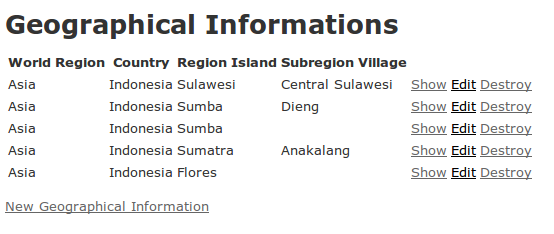
\includegraphics[scale=0.43]{index.png}
	\end{figure}
  \end{block}
\end{frame}

\begin{frame}[fragile]
  \begin{block}{GeographicalInformation Show}
	\begin{figure}
		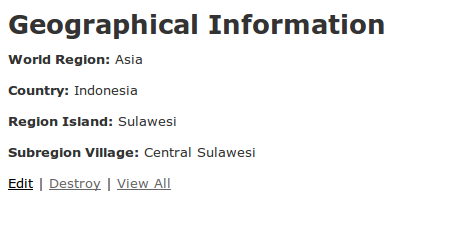
\includegraphics[scale=0.43]{show.png}
	\end{figure}
  \end{block}
\end{frame}

\begin{frame}[fragile]
  \begin{block}{GeographicalInformation Edit}
	\begin{figure}
		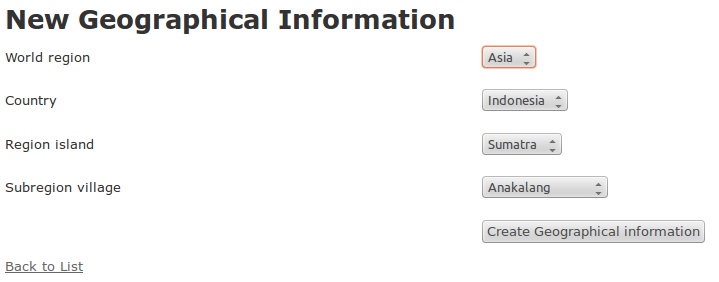
\includegraphics[scale=0.43]{edit.png}
	\end{figure}
  \end{block}
\end{frame}

\mynewsection{Documentation}

\begin{frame}
	\begin{block}{Documentation}
	\begin{itemize}
	  \item \url{http://rubyonrails.org/}
	  \item \url{http://railscasts.com/}
	  \item \url{http://railsapi.com/doc/rails-v3.2.6/}
	\end{itemize}
	\end{block}
\end{frame}

\end{document}
